\chapter{Практическая часть}


\section{Интеграция системы автоматической сборки Gradle}

\subsection{Организация проекта Gradle для проекта аналитики исторических данных}

Структурирование исходного кода и процесса сборки программных проектов играют важную роль в
обеспечении их читаемости и управляемости.
На основе накопленного опыта были выработаны оптимальные
методики, способствующие достижению этих целей.
В данном разделе рассматриваются эффективные
практики организации проектов, направленные на обеспечение их структурной ясности и удобства
сопровождения.
Также анализируются распространенные проблемы, с которыми сталкиваются разработчики,
и предлагаются методы их предотвращения.

\subsubsection{Разделение файлов исходного кода для определенных языков}

Плагины для языка Gradle устанавливают определенные соглашения относительно организации и обработки
исходного кода проекта.
Например, при использовании языка программирования Java проект автоматически
компилирует
свой исходный код, расположенный в каталоге `src/main/java`.
Аналогично, плагины для других языков
следуют подобной схеме, определяя местоположение исходных файлов в соответствии с соответствующими
соглашениями~\cite{plugin_java}.

Некоторые компиляторы способны осуществлять кросс-компиляцию для нескольких языков, используя единый
каталог для хранения исходных файлов.
В контексте оптимизации производительности сборочных
процессов, Gradle рекомендует строго соблюдать
разделение исходных файлов по языкам программирования, что облегчает как процесс сборки, так и
обеспечивает четкость в предполагаемых структурах
проекта~\cite{organize_gradle_project}.

Представленная структура исходного кода включает в себя отдельные каталоги для файлов на Java и
Kotlin.
Файлы на Java размещаются в каталоге \texttt{src/main/java}, в то время как файлы на Kotlin
хранятся
в каталоге \texttt{src/main/kotlin}.


\dirtree{%
    .1 .
    .2 build.gradle.kts.
    .2 src.
    .3 main.
    .4 java.
    .5 ParserControlller.java.
    .4 kotlin.
    .5 SocketUtils.kt.
}

\subsubsection{Тестирование}

В рамках программного проекта часто требуется проведение разнообразных видов тестирования, таких как
модульные, интеграционные, функциональные и smoke тесты.
Для эффективного управления исходным
кодом каждого типа теста рекомендуется его хранение в специально выделенных каталогах.
Практика
размещения тестового кода в отдельных каталогах положительно сказывается на удобстве сопровождения
проекта и разделении обязанностей, поскольку позволяет запускать различные типы тестов независимо
друг от друга.
Такой подход способствует повышению гибкости и эффективности процесса разработки,
облегчая выявление и устранение дефектов в приложении~\cite{test_gradle}.

В частности, мы добавляем плагин соглашения, чтобы `buildSrc` разделить настройку интеграционного
теста между несколькими подпроектами:

\begin{lstlisting}
    //...
val integrationTestTask = tasks.register<Test>("integrationTest") {
    description = "Runs integration tests."
    group = "verification"
    useJUnitPlatform()

    testClassesDirs = integrationTest.output.classesDirs
    classpath = configurations[integrationTest.runtimeClasspathConfigurationName] + integrationTest.output

    shouldRunAfter(tasks.test)
}
//...
\end{lstlisting}


Применение в проекте конкретного приложения:

\begin{lstlisting}
dependencies {
    implementation(project(":list"))
}
\end{lstlisting}

\subsubsection{Использование buildSrc для инкапсуляции императивной логики}

Для абстрагирования императивной логики в процессе сборки рекомендуется использовать
механизм `buildSrc`.
Комплексная логика сборки часто является целесообразным кандидатом для
инкапсуляции в виде пользовательской задачи или двоичного плагина.
Реализации таких пользовательских
задач и плагинов не следует размещать внутри сценариев сборки.
Использование `buildSrc` для этой
цели является предпочтительным, поскольку это позволяет избежать повторного использования кода в
различных независимых проектах.

Каталог `buildSrc` рассматривается как встроенный проект сборки.
При обнаружении этого каталога
Gradle автоматически компилирует и тестирует его содержимое, а затем включает скомпилированные
классы в путь вашего сценария сборки.
Для многопроектных сценариев сборки может быть только один
каталог `buildSrc`, который должен располагаться в корневом каталоге проекта.
Важно отдавать
предпочтение использованию плагинов сценариев, так как они обеспечивают более простое обслуживание,
рефакторинг и тестирование
кода~\cite{sharing_logic}.

\subsection{Управление зависимостями и плагинами в Gradle}

В проекте дополнительно используется механизм централизованного управления расширением зависимостей.
Модуль позволяет указать источник версий зависимостей для каталога \texttt{libs}.
В данном случае он указывает на файл \texttt{libs.versions.toml}, содержащий информацию о версиях зависимостей.

\begin{lstlisting}
dependencyResolutionManagement {
    versionCatalogs {
        create("libs") {
            from(files("configuration/libs.versions.toml"))
        }
    }
}

include("conventions")
\end{lstlisting}

В качестве основного языка для Gradle был выбран Kotlin из-за схожести синтаксиса с Java.
В данном случае, плагин \texttt{kotlin-dsl} включается для использования Kotlin DSL в качестве основного языка для написания сборочных скриптов в Gradle во всем проекте.

Плагин Spring Boot Gradle обеспечивает поддержку Spring Boot в Gradle.
Он позволяет упаковывать исполняемые jar, запускать приложения Spring Boot и использовать управление зависимостями, предоставляемое \texttt{spring-boot-dependencies}~\cite{spring_boot_gradle}.

\begin{lstlisting}
plugins {
    kotlin("jvm") version "1.5.31"
    id("org.springframework.boot") version "2.6.4"
}

dependencies {
    implementation(libs.spring.boot.gradle.plugin)
}
\end{lstlisting}

В представленном кодовом отрывке, переменная \texttt{versionCatalog} получает доступ к расширению \texttt{VersionCatalogsExtension} и идентифицирует именованный каталог версий с названием <<libs>>.

Метод \texttt{api(platform(project(":platform"))) } добавляет зависимость от платформы проекта с именем <<:platform>>.
Это указывает на то, что весь проект будет использовать версии зависимостей, определенные в данной платформе.

\begin{lstlisting}
val versionCatalog = extensions.getByType<VersionCatalogsExtension>().named("libs")
dependencies {
    api(platform(project(":platform")))

    versionCatalog.findLibrary("lombok").ifPresent {
        compileOnly(it)
        annotationProcessor(it)
    }
}
\end{lstlisting}

Такой подход способствует стандартизации и упрощает управление зависимостями, особенно в масштабируемых и многоуровневых проектах.

\subsection{Создание пользовательских задач и скриптов в Gradle}

В проекте используется несколько пользовательских задач, переопределяющих стандартное поведение Gradle.

Директива \texttt{manifest \{\ldots \}} определяет настройки манифеста, который содержит метаданные о проекте.
В данном контексте устанавливаются атрибуты манифеста, такие как `Implementation-Title` (название реализации) и `Implementation-Version` (версия реализации), которые присваиваются соответственно имени и версии проекта.

\begin{lstlisting}
tasks.jar {
    manifest {
        attributes(
                mapOf(
                        "Implementation-Title" to project.name,
                        "Implementation-Version" to project.version
                )
        )
    }
}
\end{lstlisting}

\subsection{Оптимизация процесса сборки с использованием Gradle}

Эффективность процесса сборки играет решающую роль в производительности разработки.
Увеличение
времени сборки повышает риск прерывания рабочего процесса.
Учитывая, что сборки запускаются
многократно в течение дня, даже небольшие задержки могут существенно
накапливаться~\cite{gradle_perfomance}.

\subsubsection{Параллельное выполнение сборки}

Так как проект состоит более чем из одного подпроекта линейная сборка занимает значительное время
из-за не равносильности подпроектов.
Так как из-за микросервисной архитектуры подпроекты независимы
друг от друга, то они не имеют общего состояния.
В таком случае есть смысл заставить Gradle
выполнять сборку подпроектов параллельно.

Для этого в проекте используется флаг:

\begin{lstlisting}
    org.gradle.parallel = true
\end{lstlisting}



Результаты оптимизации представлены на рисунке~\ref{fig:parallel}:

\begin{figure}[htbp]
    \centering
    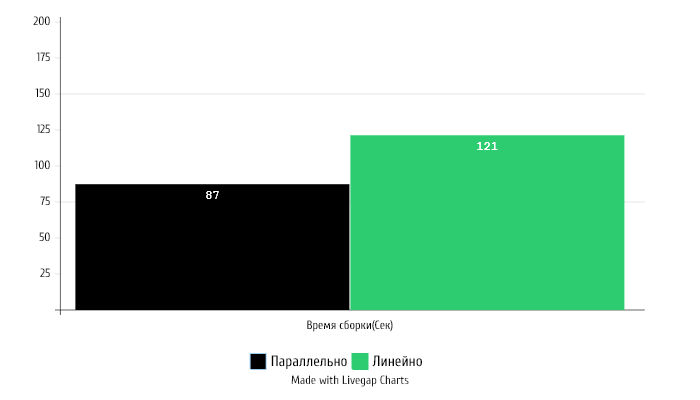
\includegraphics[width=0.8\textwidth]{parallel}
    \caption{Результат оптимизации}
    \label{fig:parallel}
\end{figure}
Прирост производительности автоматизированной сборки составил 21\%.


\section{Внедрение API Gateway}

\subsection{Анализ требований и постановка задач}

Проект начинается с определения основных требований к системе, включая:

\begin{itemize}
    \item Обеспечение высокодоступного и отказоустойчивого доступа к данным.
    \item Масштабируемость для обработки большого объема запросов.
    \item Безопасность и защита данных.
    \item Гибкость маршрутизации и обработки запросов.
\end{itemize}

\subsection{Основные компоненты архитектуры}

Архитектура системы включает следующие основные компоненты:

\begin{itemize}
    \item Spring Cloud Gateway: Центральный элемент для маршрутизации запросов и применения политик безопасности.
    \item Микросервисы: Каждый микросервис отвечает за конкретные функции, такие как обработка данных, управление пользователями, генерация отчетов и т.д.
    \item Базы данных: Хранение структурированных и неструктурированных данных о православных объектах, исторической информации и т.д.
    \item Интерфейсы пользователя: Веб-приложения и мобильные приложения для взаимодействия с пользователями.
\end{itemize}

\subsection{Описание архитектуры проекта до внедрения Spring Cloud Gateway}

До внедрения API gateway в проект аналитики исторических данных все запросы маршрутизировались напрямую каждому микросервису.

За собой это влекло ряд трудностей, которые требовали решения.
Первостепенно - это вопрос безопасности.
Прямой доступ значительно повышает вероятность потенциальных угроз.
Дополнительно это усложняет соблюдение единой политики безопасности.

Следующей трудностью оказалось версионирование API. У каждого микросервиса есть свой эндоинт, в том числе даже в рамках одного сервиса существуют разные версии конечной точки.
Возникала проблема доступа к разным версиям API\@.

Таким образом, отсутствие API Gateway приводило к множеству организационных и технических проблем, которые отрицательно сказывались на эффективности разработки, поддержке и масштабируемости системы.

Архитектурная схема работы проекта до внедрения выглядела следующим образом~\ref{fig:without_gate}.

\begin{figure}[htbp]
    \centering
    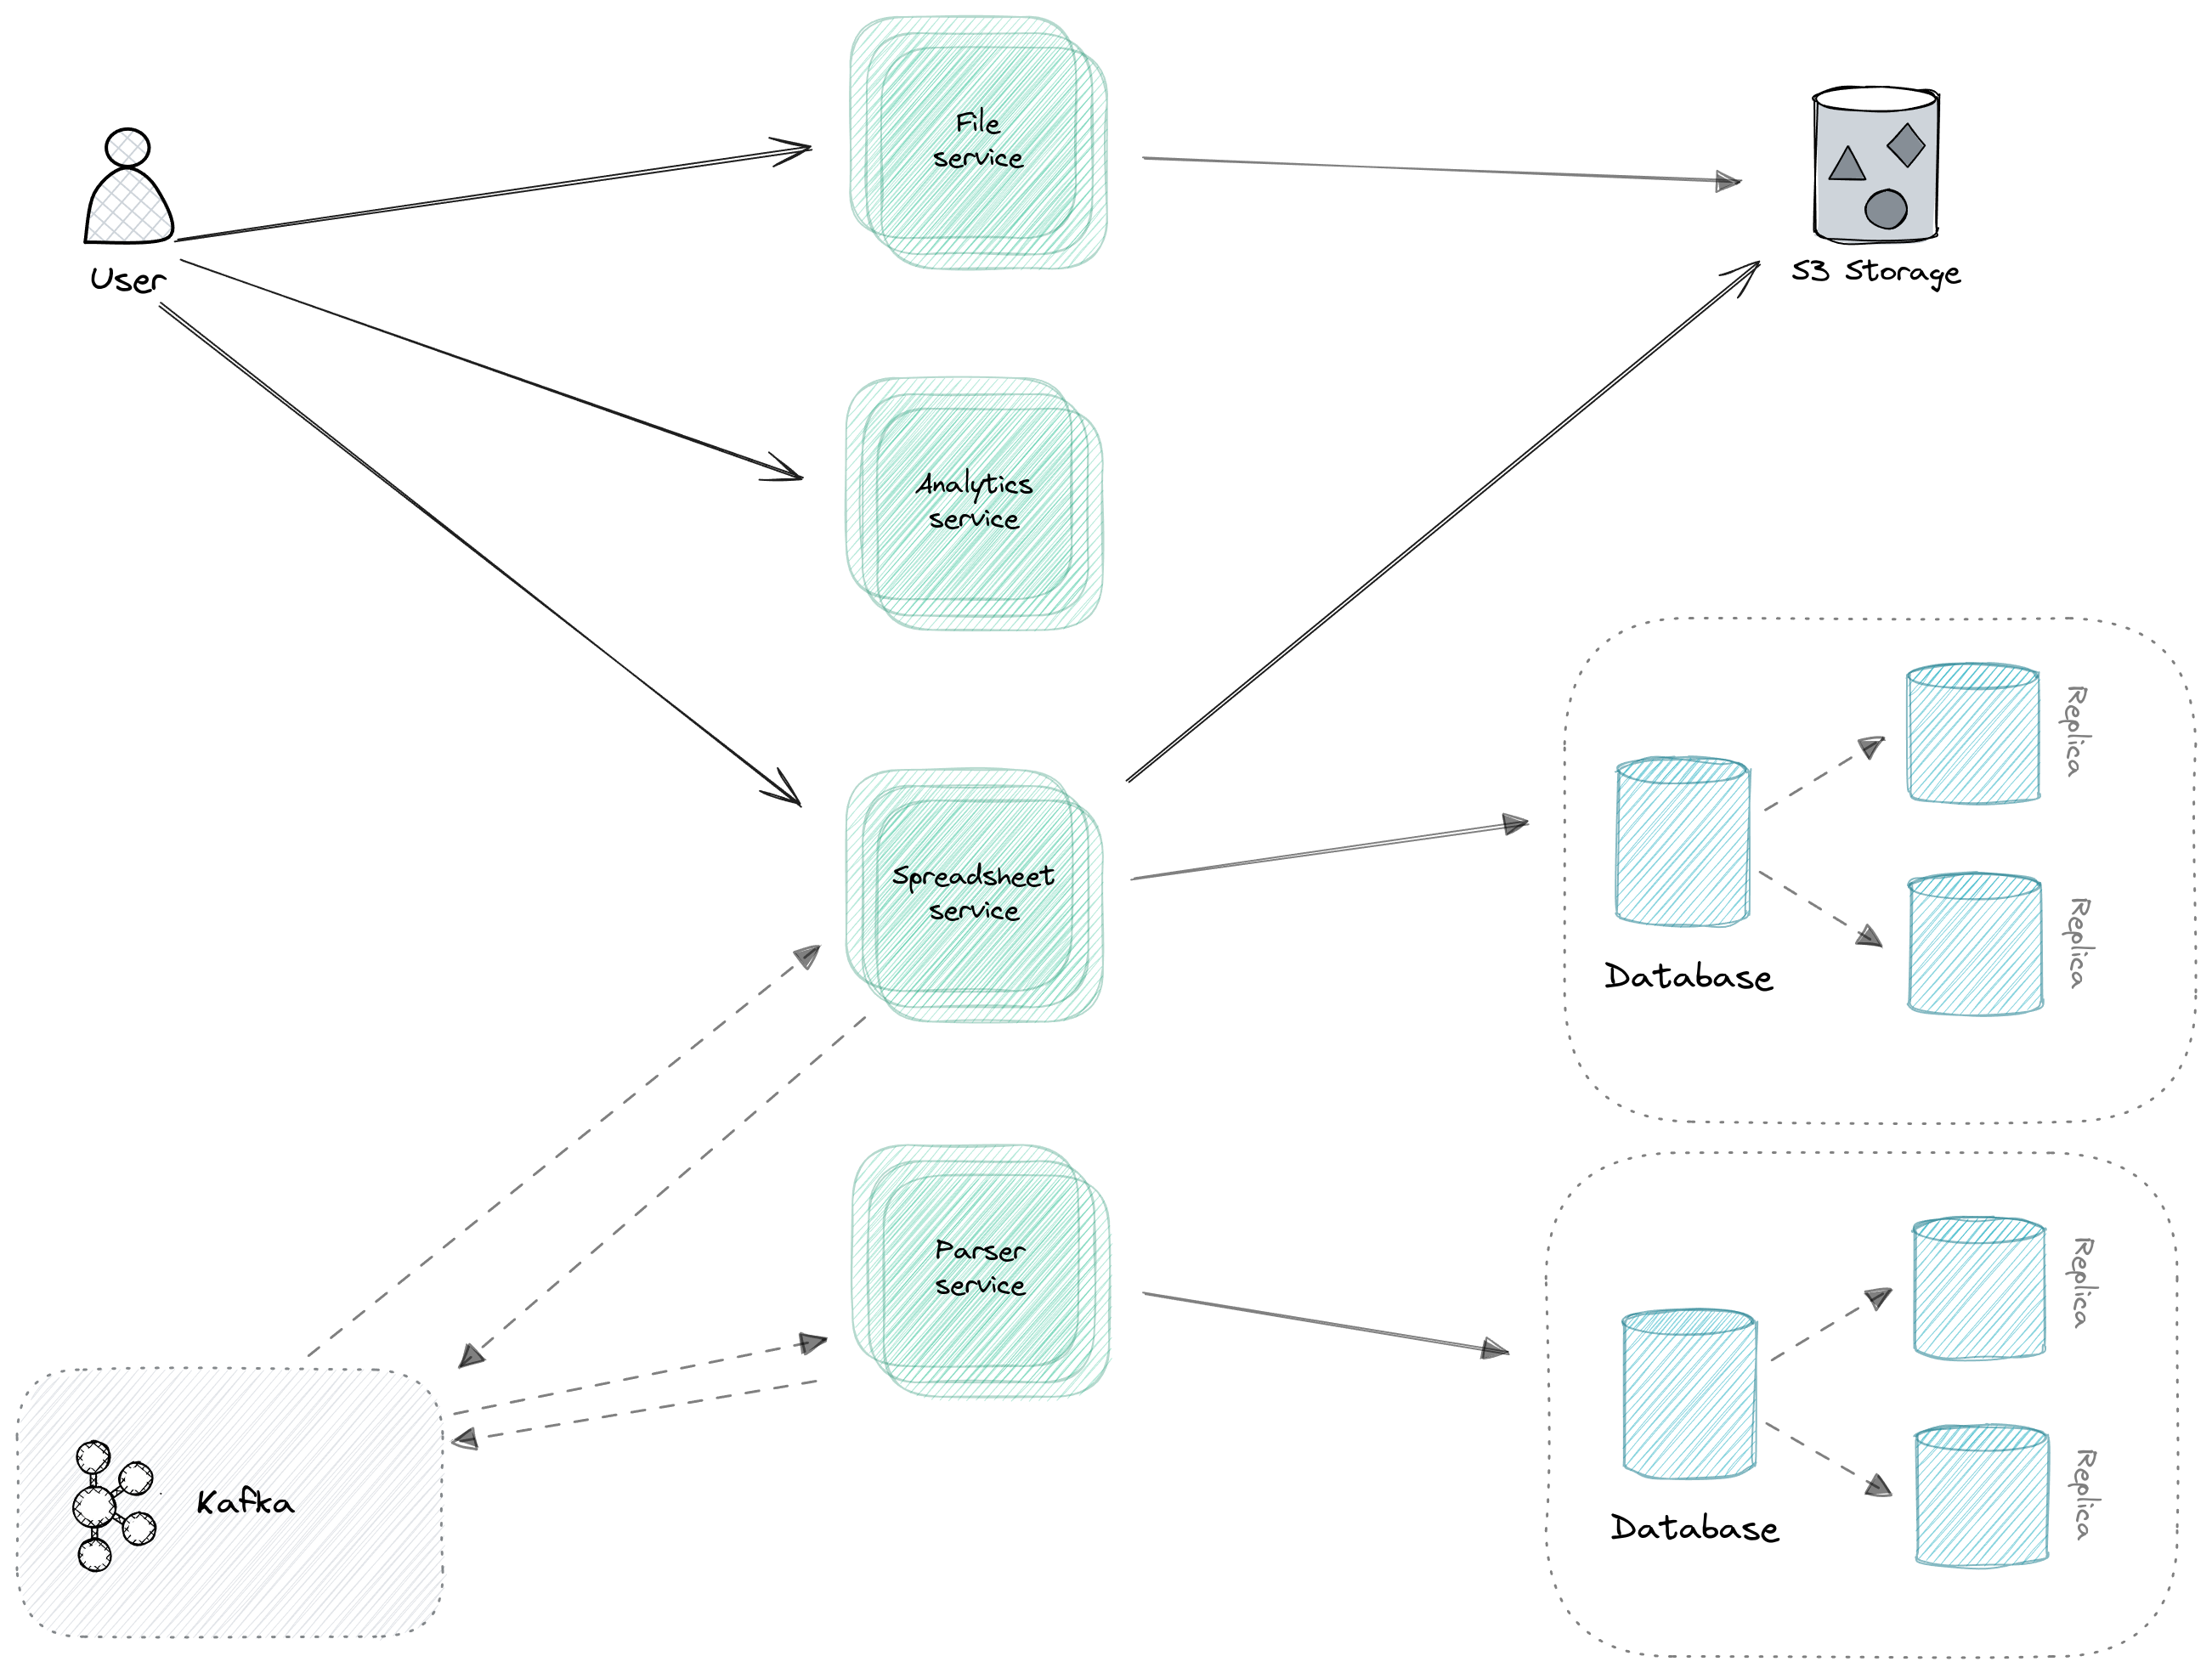
\includegraphics[width=0.8\textwidth]{img}
    \caption{Архитектура без фильтра}
    \label{fig:without_gate}
\end{figure}

\subsection{Проектирование архитектуры с использованием Spring Cloud Gateway}

В данном разделе представлена концепция проектирования архитектуры информационно-аналитического онлайн-ресурса «Православный ландшафт таежной Сибири» с использованием Spring Cloud Gateway.
Основная цель заключается в создании масштабируемой, надежной и безопасной системы для анализа и представления данных, связанных с православными объектами в таежных регионах Сибири, которая решает проблемы озвученные ранее.

В теоретической части описывались различные подходы к реализации.
Исходя из этого была выбрана модель API Gateway.

Была спроектирована схема, которая представлена на рисунке~\ref{fig:api_gateway}.

\begin{figure}[htbp]
    \centering
    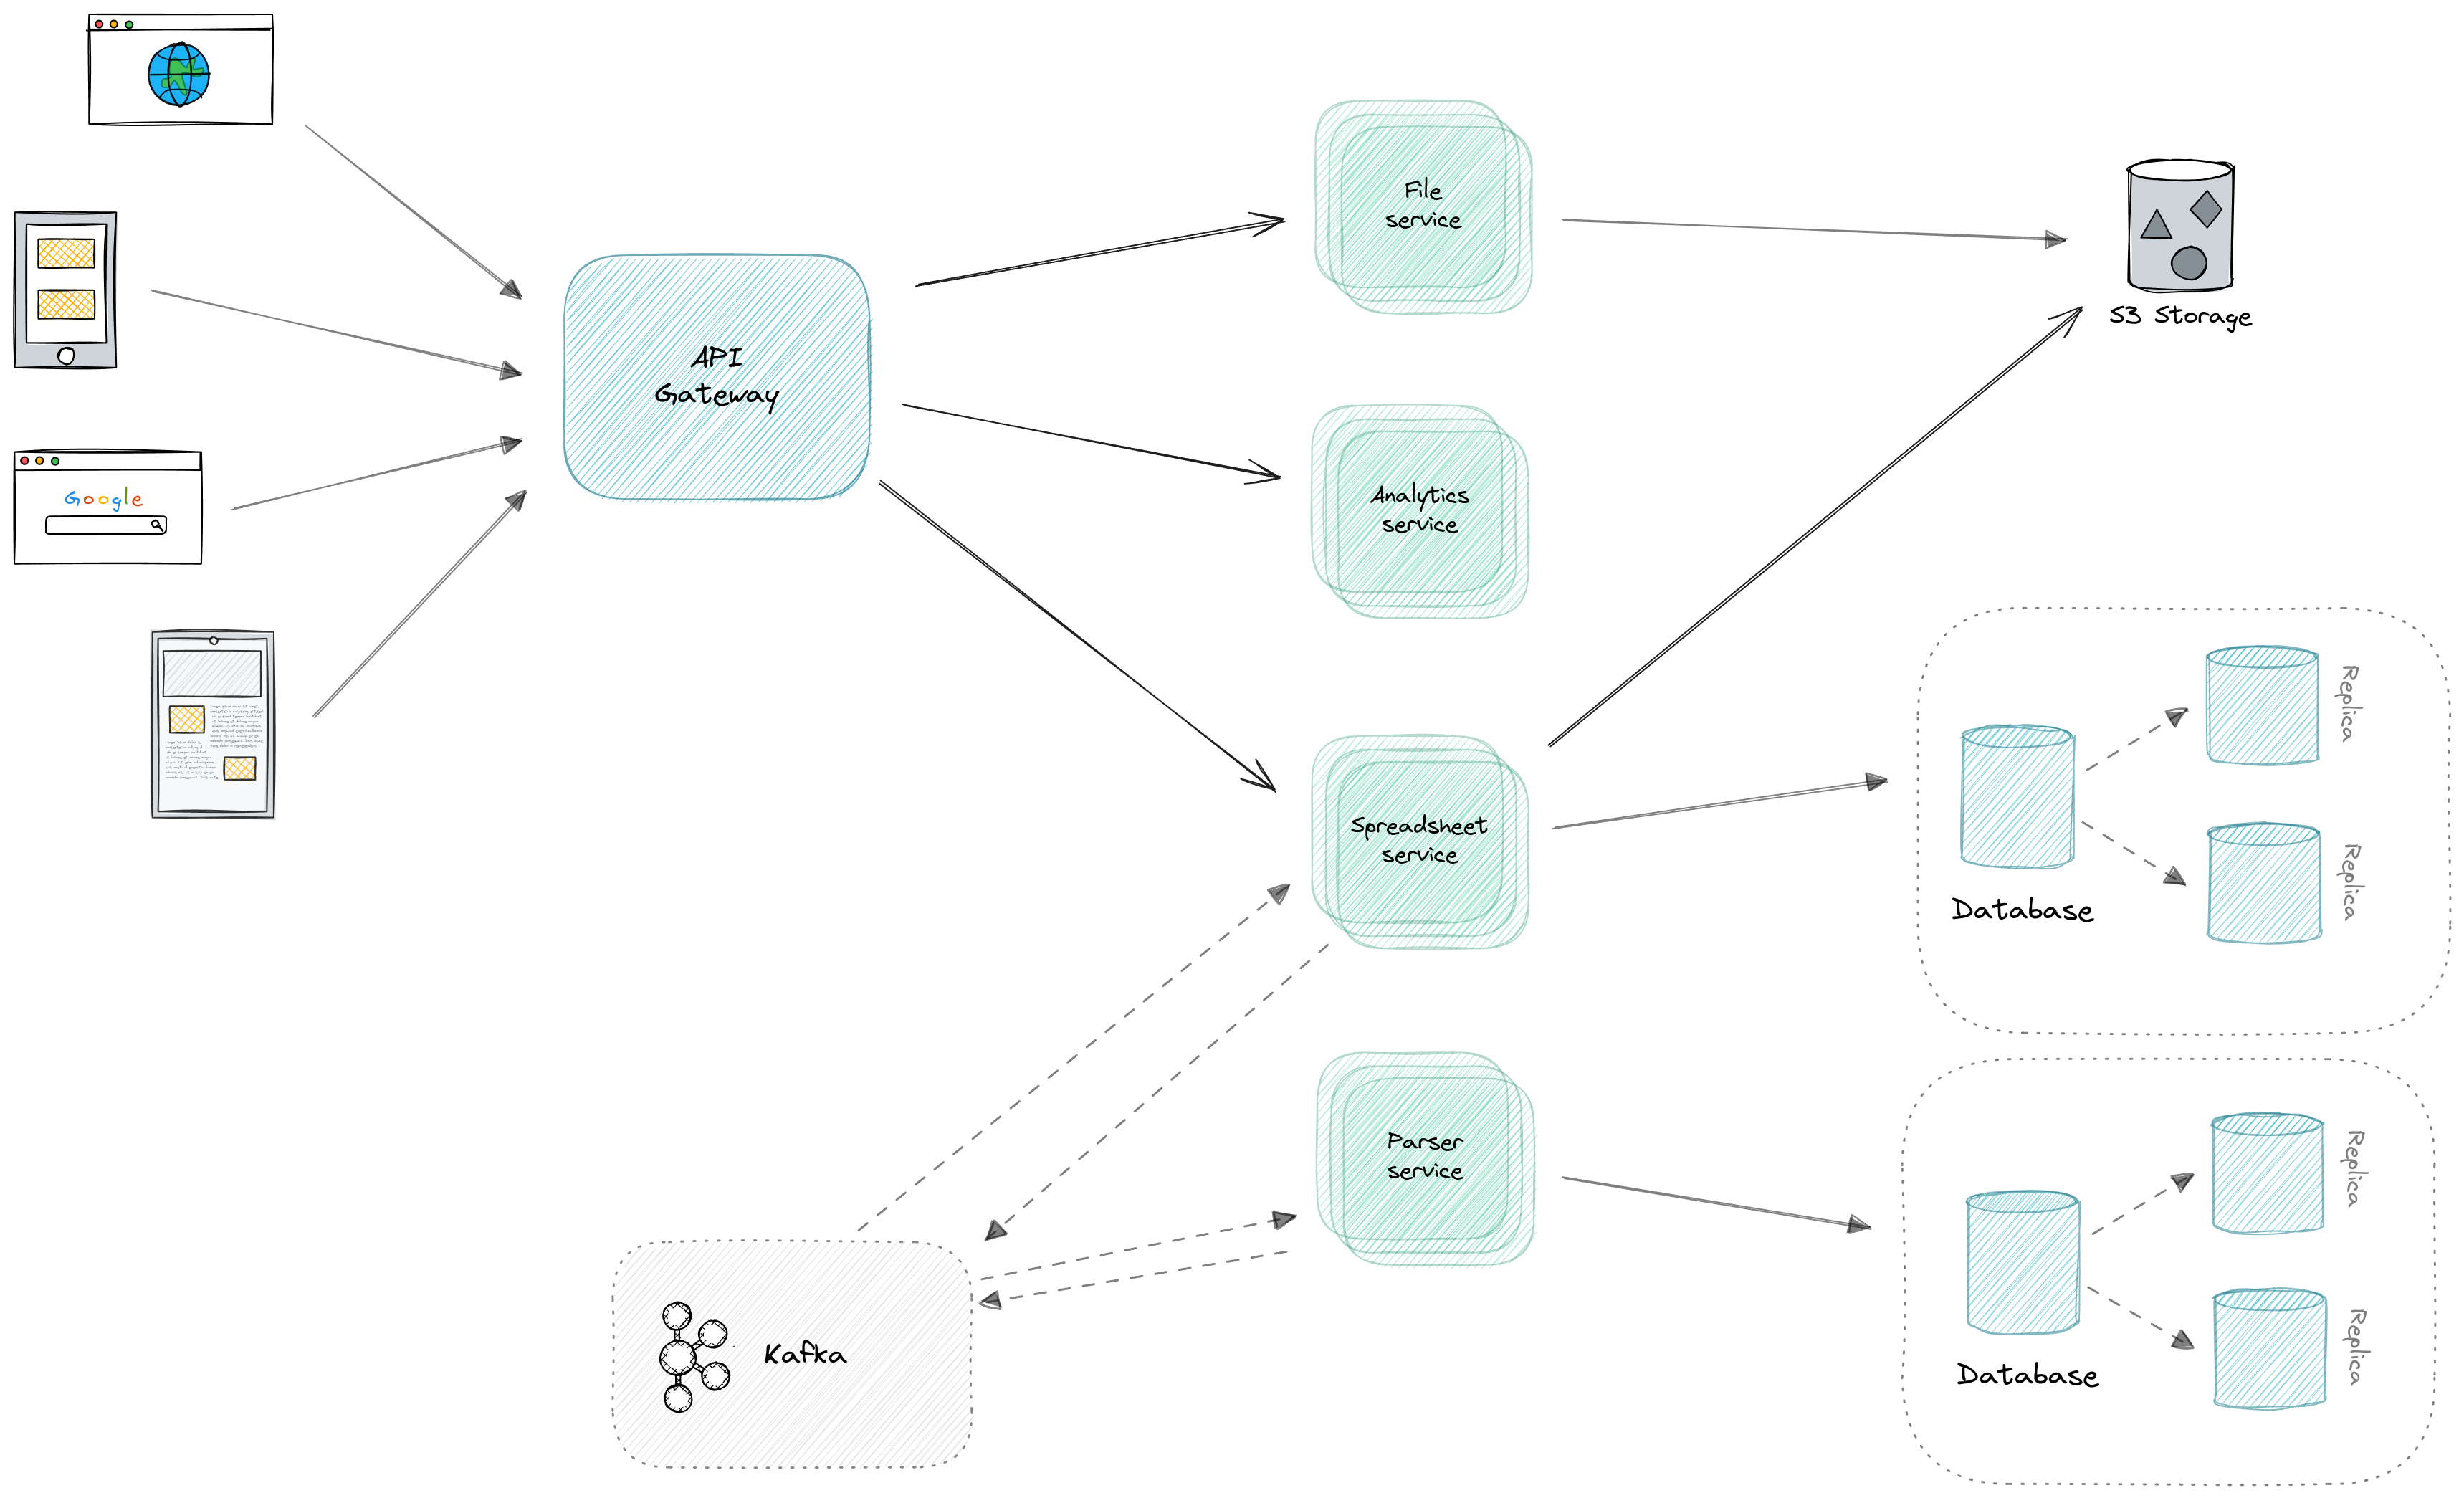
\includegraphics[width=0.8\textwidth]{api_gateway}
    \caption{Архитектура с фильтром}
    \label{fig:api_gateway}
\end{figure}

\subsection{Реализация в проекте}

Для начала необходимо сконфигурировать балансировщик нагрузки встроенный в Spring Cloud Gateway.

\begin{lstlisting}[language=java]
public class LoadBalancerConfiguration {

    @Bean
    ReactorLoadBalancer<ServiceInstance> roundRobinLoadBalancer(
            Environment environment,
            LoadBalancerClientFactory loadBalancerClientFactory
    ) {
        String name = environment.getProperty(LoadBalancerClientFactory.PROPERTY_NAME);
        return new RoundRobinLoadBalancer(
                loadBalancerClientFactory.getLazyProvider(name, ServiceInstanceListSupplier.class),
                name
        );
    }
}
\end{lstlisting}

Балансировщик нагрузки RoundRobinLoadBalancer реализует алгоритм кругового перебора (Round Robin), распределяя входящие запросы равномерно между доступными экземплярами сервиса.

Таким образом, данный метод конфигурирует и возвращает балансировщик нагрузки, который использует алгоритм кругового перебора для распределения нагрузки между экземплярами сервиса в зависимости от имени сервиса, указанного в свойствах окружения.

Далее идет настройка маршрутизации и фильтрации.

\begin{lstlisting}
//.....
@Bean
public RouteLocator customRouteLocator(RouteLocatorBuilder builder) {
    return builder.routes()
            .route(SIMPLE_RES_ID, r -> r
                    .path(SIMPLE_RES_PATH)
                    .filters(f -> f
                            .rewritePath(API_PATH, "")
                    )
                    .uri(loadBalancerUriFor(serviceConfig.getSimple()))
            ).
    //......
}
\end{lstlisting}

\subsection{Внедрение SSL сертификатов}

Подготовка SSL сертификата.
Необходимо приобрести SSL сертификат у доверенного центра сертификации (CA) через Госуслуги можно бесплатно получить электронный сертификат безопасности — стандартный OV или базовый DV

Сертификат от Минцифры заменит иностранный в случае его отзыва или окончания срока действия, или создать самоподписанный сертификат.
Для создания самоподписанного сертификата можно воспользоваться инструментами, такими как `keytool` или `openssl`.
Например, для создания сертификата с использованием `keytool`:

\begin{lstlisting}
keytool -genkeypair -alias myalias -keyalg RSA -keysize 2048 -storetype PKCS12 -keystore keystore.p12 -validity 3650
\end{lstlisting}

Этот процесс создаст файл хранилища ключей `keystore.p12`, который будет использоваться в приложении.

Настройка Spring Boot для использования SSL сертификата.
В проекте Spring Boot необходимо настроить файл конфигурации `application.yml` для использования SSL. Пример настройки в файле `application.yml`:

\begin{lstlisting}
server:
  port: 8443
  ssl:
    key-store: classpath:keystore.p12
    key-store-password: your_password
    key-store-type: PKCS12
    key-alias: myalias
\end{lstlisting}

В данной конфигурации указывается путь к хранилищу ключей, его пароль, тип хранилища и алиас ключа.

Обновление конфигураций клиента.
Все клиентские приложения, обращающиеся к вашему API Gateway, должны быть обновлены для использования HTTPS вместо HTTP. Это включает изменение URL-адресов в конфигурационных файлах или коде приложений, а также проведение тестирования для проверки корректности работы.

Таким образом, выполнение вышеуказанных шагов позволяет успешно внедрить SSL конфигурации в Spring Cloud API Gateway, обеспечивая безопасность данных и защищенные соединения между клиентами и сервером.


\section{Проектирование архитектуры проекта с учетом сервера конфигурации}

Проектирование архитектуры сервера конфигурации позволяет централизованно управлять конфигурационными данными,
обеспечивая их консистентность и безопасность.
Это упрощает администрирование, повышает надежность системы и позволяет
быстро адаптироваться к изменениям без необходимости перезапуска приложений.

\subsection{Схема взаимодействия компонентов}

В ходе работы была спроектированная схема, представленная на рисунке~\ref{fig:config}

\begin{figure}[htbp]
    \centering
    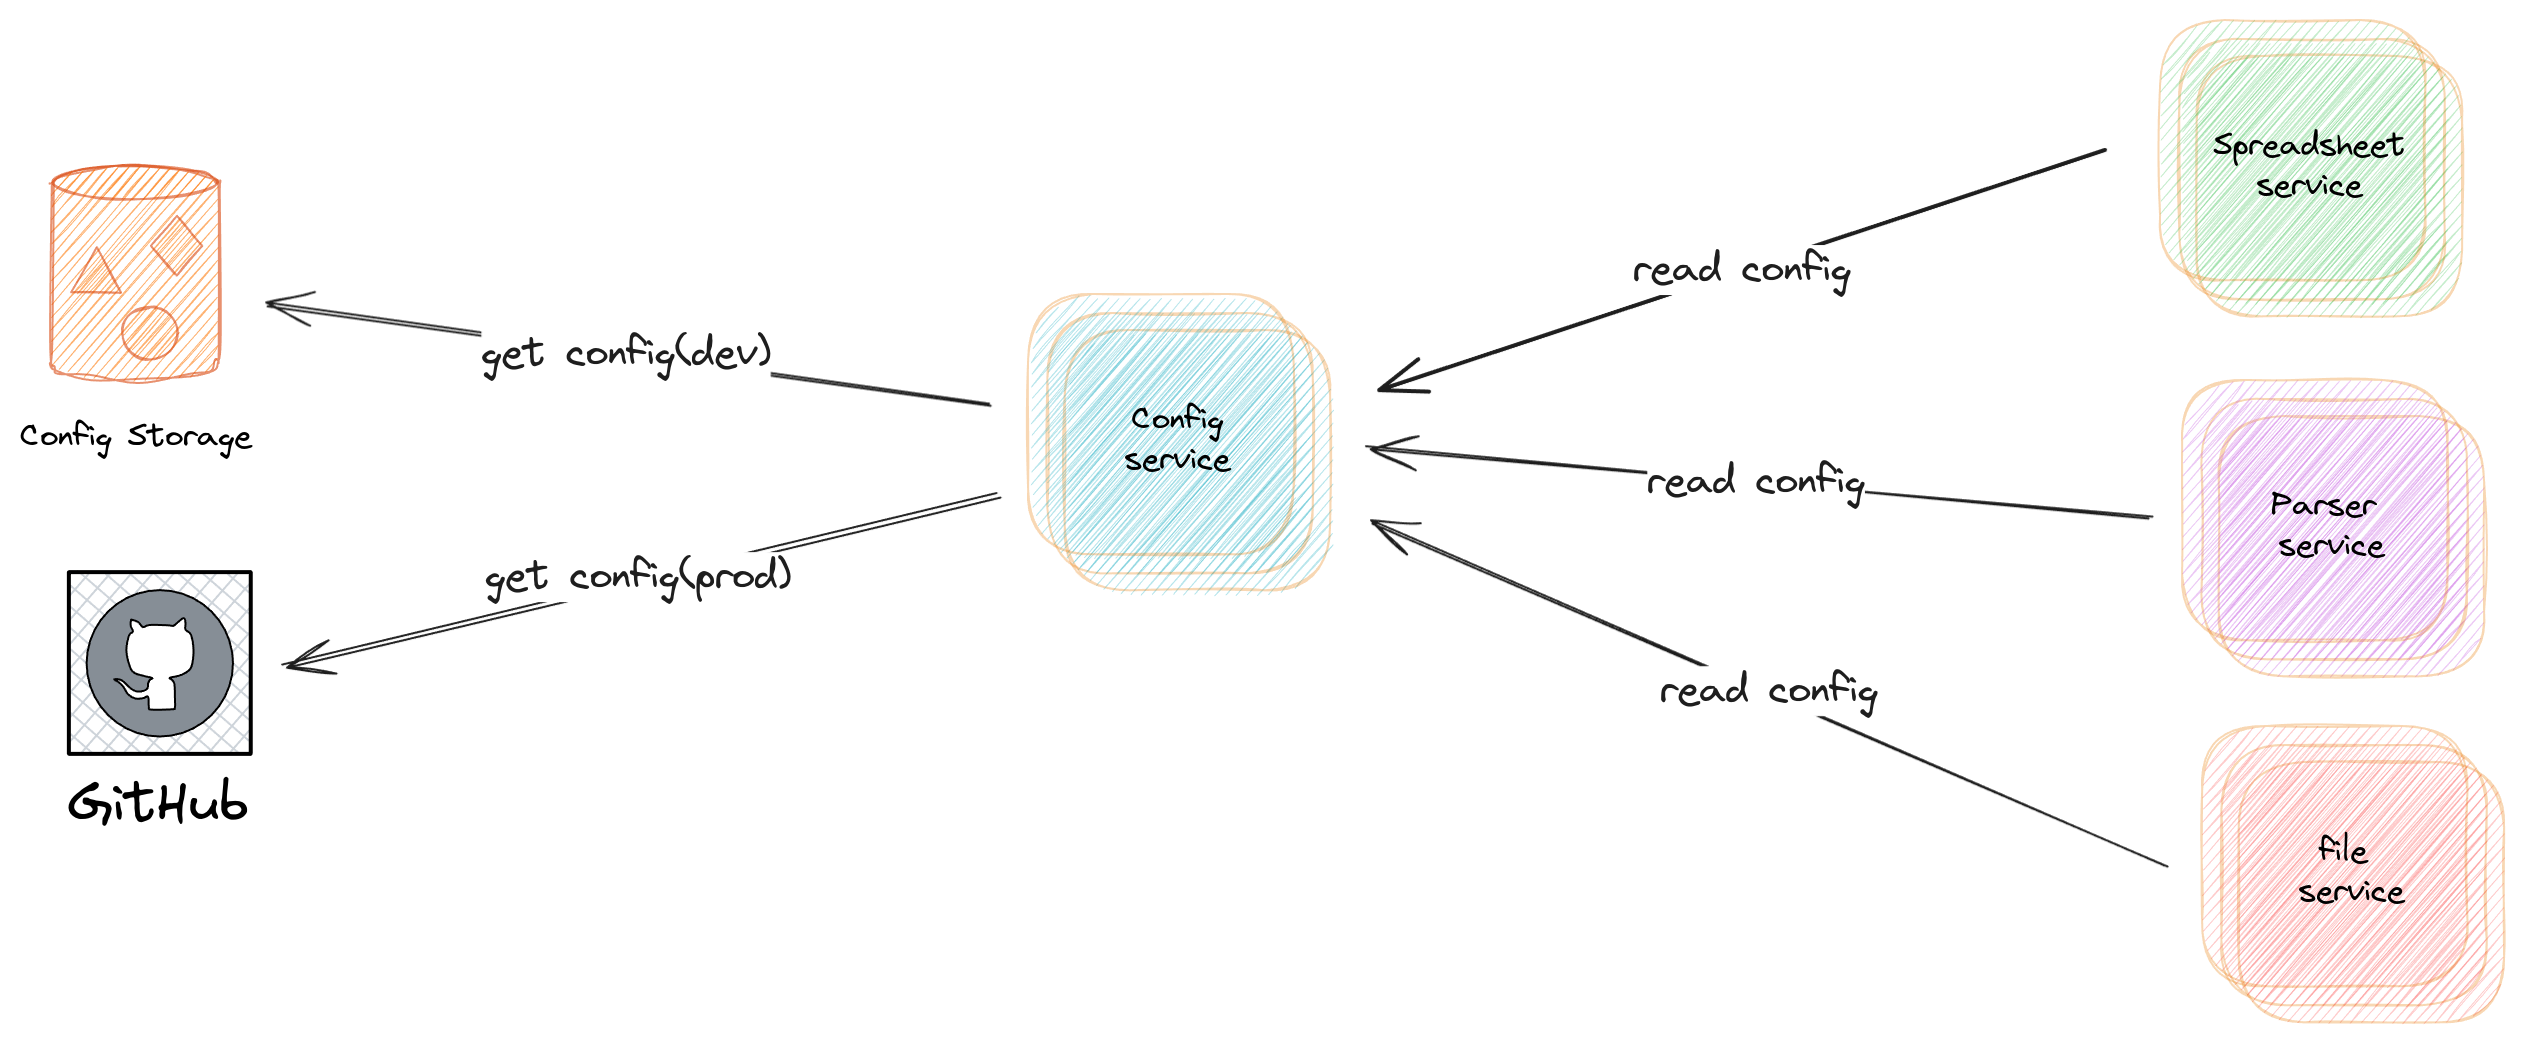
\includegraphics[width=0.8\textwidth]{img_1}
    \caption{Config service}
    \label{fig:config}
\end{figure}

Благодаря такому подходу мы можем разделить конфигурации для
среды разработки приложения и настоящей.

\subsection{Безопасность и контроль доступа}

Spring Cloud Config предоставляет возможности для реализации различных механизмов безопасности и контроля доступа,
которые обеспечивают защиту конфигурационных данных от несанкционированного доступа и изменений.
Аутентификация пользователей и сервисов, получающих доступ к Spring Cloud Config, является первым шагом в обеспечении
безопасности.
Spring Cloud Config поддерживает различные методы аутентификации.
Он из <<коробки>> интегрируется с различными провайдерами OAuth2, такими как Auth0, Okta, Keycloak.

Защита конфиденциальных конфигурационных данных, таких как учетные данные и ключи API, осуществляется с помощью
шифрования.
Spring Cloud Config поддерживает шифрование конфиденциальных значений в конфигурационных файлах.
Для этого используются
такие инструменты, как JCE (Java Cryptography Extension) и внешние сервисы шифрования (например, HashiCorp Vault).
Использование TLS (Transport Layer Security) для шифрования данных при передаче между клиентами и сервером Spring Cloud
Config, что защищает данные от перехвата и манипуляций.

\subsection{Репликация и отказоустойчивость}

Для обеспечения отказоустойчивости Spring Cloud Config Service следует применять несколько стратегий:
Развертывание нескольких экземпляров Spring Cloud Config Server в кластерной конфигурации с использованием
балансировщика нагрузки, который будет распределять запросы между доступными
экземплярами.
Это обеспечивает устойчивость к сбоям отдельных узлов.
Использование нескольких зеркальных копий конфигурационных хранилищ (Git-репозиториев или баз данных) с автоматическим
переключением на доступный репозиторий в случае сбоя основного хранилища.
Локальное кеширование конфигурационных данных на уровне клиентских приложений с использованием механизма Spring Cloud
Config Client.
В случае недоступности конфигурационного сервера клиент может временно использовать закешированные
данные.

\subsection{Интеграция сервера конфигурации с микросервисами}

\subsection{Настройка подключения микросервисов к серверу конфигурации}

Интеграция сервиса конфигурации прошла успешно.
Для этого были приняты несколько шагов.
В целях безопасности далее реальные наименования и данные будут заменены на условные.

Реализация EnvironmentRepository по умолчанию использует серверную часть \texttt{Git}, что чрезвычайно удобно для управления обновлениями и физическими средами, а также для аудита изменений.
Чтобы изменить расположение репозитория, можно настроить свойство конфигурации \texttt{spring.cloud.config.server.git.uri} на сервере конфигурации, например, в файле \texttt{application.yml}.
При установке этого свойства с префиксом \texttt{file:} репозиторий будет работать из локального хранилища, что позволяет быстро и легко начать работу без необходимости запуска сервера.
В данном случае сервер будет работать непосредственно с локальным репозиторием, не клонируя его, что не зависит от его публичного статуса, поскольку сервер конфигурации никогда не изменяет `удалённый` репозиторий.

\subsubsection{SSL сертификация}

В зависимости от назначения развертывания используются разные параметры для SSL сертификатов.

\begin{verbatim}
spring:
  cloud:
    config:
      server:
        git:
          uri: https://www.ru/my/git_repo
          skipSslValidation: true/false
\end{verbatim}

Spring Cloud Config Server поддерживает URL-адрес репозитория git с заполнителями для параметров \{application\} и \{profile\}.
Это позволяет реализовать политику «один репозиторий на приложение», используя структуру, аналогичную следующей.

\begin{verbatim}
uri: https://github.com/myorg/{application}
\end{verbatim}

\subsubsection{Безопасность}

Для использования базовой аутентификации HTTP в удалённом репозитории необходимо отдельно указать свойства имени пользователя и пароля, а не включать их в URL. Пример конфигурации представлен ниже:

\begin{verbatim}
spring:
  cloud:
    config:
      server:
        git:
          uri: https://github.com/config-repo
          username: user
          password: user
\end{verbatim}

Если не используется HTTPS и учётные данные пользователя, можно использовать SSH, при условии, что ключи хранятся в стандартных директориях (\textasciitilde{}/.ssh), а URI указывает на SSH-адрес, например, <git@github.com>: configuration/cloud-configuration.
Важно, чтобы в файле \textasciitilde{}/.ssh/known\_hosts содержалась запись для Git-сервера в формате ssh-rsa, так как другие форматы (например, ecdsa-sha2-nistp256) не поддерживаются.
Для избежания непредвиденных проблем следует убедиться, что в файле known\_hosts присутствует только одна запись для Git-сервера, соответствующая указанному в конфигурационном сервере URL. Если в URL используется имя хоста, оно должно точно совпадать с записью в known\_hosts, а не с IP-адресом.
Репозиторий доступен через JGit.
Настройки HTTPS-прокси могут быть заданы в файле \textasciitilde{}/.git/config или с помощью системных свойств JVM (-Dhttps.proxyHost и -Dhttps.proxyPort).

Если удалённые источники свойств содержат зашифрованное содержимое (значения, начинающиеся с \{cipher\}), они расшифровываются перед отправкой клиентам по HTTP. Основным преимуществом данной настройки является то, что значения свойств не обязательно должны быть в открытом виде, когда они находятся «в покое» (например, в репозитории Git).
Если значение не может быть расшифровано, оно удаляется из источника свойств, и добавляется дополнительное свойство с тем же ключом, но с префиксом invalid и значением, означающим «не применимо» (обычно <n/a>).
Это делается в основном для предотвращения случайного использования зашифрованного текста в качестве пароля и его утечки.

Если настроен удалённый репозиторий конфигурации для клиентских приложений конфигурации, он может содержать файл application.yml, аналогичный следующему:

\begin{verbatim}
spring:
  datasource:
    username: dbuser
    password: '{cipher}123123ASDASDQWEQWE'
\end{verbatim}

Эти значения можно безопасно отправить в общий репозиторий Git, и секретный пароль останется защищённым.

Сам же доступ к конфигурации можно получить только имея необходимые права и скоупы для протокола OAuth 2.0.

\subsubsection{Перспективы развития}

В перспективе развития данной технологии возможно углубление интеграции с современными инструментами управления
конфигурациями, такими как Vault, а также расширение функциональности для
обеспечения более гибкого управления версиями конфигураций и автоматизации процессов развертывания и обновления
приложений.
Не исключается вариант перехода на Etcd.
